\documentclass{article}
\usepackage{graphicx}
\usepackage{float}

\begin{document} 
\begin{center}
{\bf \Large  Homework 4} \\
\end{center}
Chien-Pin Chen\\
05/09/2016\\

\noindent {\bf Problem 1.} A linear system describing the dynamics of 
$x_1(k)$ and $x_2(k)$ can be written as

\begin{eqnarray}
  x_1(k+1) &=& x_1(k)-0.8x_1(k)+0.4x_2(k)+w_1(k) \\
  x_2(k+1) &=& x_2(k)-0.4x_1(k)+1+w_2(k) 
\end{eqnarray}

\noindent where $w_1(k)$, $w_2(k)$ are zero-mean value independent Gaussian random 
variables with variance 1. The initial expected values are $\overline{x}_1(0) = 10$, 
$\overline{x}_2(0) = 20$ and the covariance matrix of the vector $x(0) = [x_1(0)\ x_2(0)]^T$
is $P(0) = diag(40, 40)$. Plot the evolution of the expected values for $k=0..14$. In a separate figure, plot the evolution of the variance corresponding to $x_1(k)$ and the one corresponding to $x_2(k)$, $k=0..14$.  \\ \\
ANS:\\
Equation 1 and  2 can rewrite as:

\begin{eqnarray}
	\left[ {\begin{array}{*{20}c}
	   {x_1 (k + 1)}  \\
	   {x_2 (k + 1)}  \\
	\end{array}} \right] = \left[ {\begin{array}{*{20}c}
	   {0.2} & {0.4}  \\
	   { - 0.4} & 1  \\
	\end{array}} \right]\left[ {\begin{array}{*{20}c}
	   {x_1 (k)}  \\
	   {x_2 (k)}  \\
	\end{array}} \right] + \left[ {\begin{array}{*{20}c}
	   1 & 0  \\
	   0 & 1  \\
	\end{array}} \right]\left[ {\begin{array}{*{20}c}
	   {w_1 (k)}  \\
	   {w_2 (k)}  \\
	\end{array}} \right] + \left[ {\begin{array}{*{20}c}
	   0  \\
	   1  \\
	\end{array}} \right]
\end{eqnarray}

And, the expected values of $x(0) = [x_1(k)\ x_2(k)]^T$ is:

\begin{eqnarray}
	E\left\{ {\left[ {\begin{array}{*{20}c}
	   {x_1 (k + 1)}  \\
	   {x_2 (k + 1)}  \\
	\end{array}} \right]} \right\} = \left[ {\begin{array}{*{20}c}
	   {0.2} & {0.4}  \\
	   { - 0.4} & 1  \\
	\end{array}} \right]E\left\{ {\left[ {\begin{array}{*{20}c}
	   {x_1 (k)}  \\
	   {x_2 (k)}  \\
	\end{array}} \right]} \right\} + \left[ {\begin{array}{*{20}c}
	   0  \\
	   1  \\
	\end{array}} \right]\\
	\left[ {\begin{array}{*{20}c}
	   {\bar x_1 (k + 1)}  \\
	   {\bar x_2 (k + 1)}  \\
	\end{array}} \right] = \left[ {\begin{array}{*{20}c}
	   {0.2} & {0.4}  \\
	   { - 0.4} & 1  \\
	\end{array}} \right]\left[ {\begin{array}{*{20}c}
	   {\bar x_1 (k)}  \\
	   {\bar x_2 (k)}  \\
	\end{array}} \right] + \left[ {\begin{array}{*{20}c}
	   0  \\
	   1  \\
	\end{array}} \right]
\end{eqnarray}
Using equation 5 with the initial values $\overline{x}_1(0) = 10$, $\overline{x}_2(0) = 20$ to plot 
the evolutions of expected value for (time step) $k=0..14$ in MATLAB:\\\\

For $\overline{x}(k)$:
\begin{figure}[H]
\begin{center}
	\includegraphics[scale=0.5]{figure/hw4_ex12.jpg}
	\caption{The evolution of expected values of $ x(k) $}
\end{center}
\end{figure}


Next, for the variance of $x_1(k)$ and $x_2(k)$, I use equation:\\
\begin{equation}
	P_{k + 1}  = AP_k A^T  + \Gamma Q\Gamma ^T 
\end{equation}
with initial value:\\
\begin{equation}
	P_0  = \left[ {\begin{array}{*{20}c}
	   {40} & 0  \\
	   0 & {40}  \\
	\end{array}} \right]
\end{equation}
and covariance matrix:
\begin{equation}
	Q = \left[ {\begin{array}{*{20}c}
	   1 & 0  \\
	   0 & 1  \\
	\end{array}} \right]
\end{equation}
to plot the evolution of variance of $x_1(k)$ and $x_2(k)$ for (time step) $k=0..14$ in MATLAB:\\\\
For the covariance of $x(k)$:
\begin{figure}[H]
\begin{center}
	\includegraphics[scale=0.5]{figure/hw4_varx12.jpg}
	\caption{The evolution of variance of $ x(k) $}
\end{center}
\end{figure}


\noindent {\bf Problem 2.} While moving, the position and velocity of a university campus bus along its route are described by the following stochastic differential equation
\begin{eqnarray}
  ds &=& vdt \\
  dv &=& -2vdt+22dt+20dw 
\end{eqnarray}

\noindent where $s(t)$ is the distance traveled along the route and $v(t)$ is the bus velocity. The initial position of the bus at $t = 0$ is known with the variance $var(s(0)) =100$ and the velocity variance corresponds to its value at the steady state, i.e.,
$var(v(0)) = \lim_{t \rightarrow \infty} var(v(t))$. The variables $s(0)$ and $v(0)$ are 
independent at the time point $t = 0$. At what point of time $t^*$, the variance $var(s(t^*)) = 2var(s(0))$? Provide differential equations describing dynamics of the variances, derive the steady state of $var(v(t))$ and explain your conclusions. Numerical solutions are accepted.\\
ANS:\\
First, I derive the steady state of the variance of $v(t)$. For linear stochastic differential equation (such as equation 10) could express as:\\
\begin{equation}
	dx(t) = Ax(t)dt + udt + bdw
\end{equation}
Then, A is -2, b is 20, and u is 22 in equation 10.\\
Next, I could use equation:\\
\begin{equation}
	\dot P = PA^T  + AP + bb^T 
\end{equation}
to compute the derivative of the variance of $v(t)$ :
\begin{eqnarray}
	\dot \sigma _{v(t)}^2  = \,\, - 2 \times \sigma _{v(t)}^2  + \sigma _{v(t)}^2  \times  - 2 + 20 \times 20\\
	\dot \sigma _{v(t)}^2  = \,\, - 4\sigma _{v(t)}^2  + 400
\end{eqnarray}
At steady state, when $t \to \infty$, I could  assume that $\dot \sigma _{v(\infty )}^2  \to 0$ and $\sigma _{v(\infty )}^2  = \sigma _{v(0)}^2$.\\
Then from equation 14, I could get:
\begin{eqnarray}
	\underbrace {\dot \sigma _{v(\infty )}^2 }_0 = \,\, - 4\underbrace {\sigma _{v(\infty )}^2 }_{\sigma _{v(0)}^2 } + 400\\
	\sigma _{v(0)}^2  = 100
\end{eqnarray}
Next, I could also rewrite equation 9 and 10 as equation 11:
\begin{equation}
	d\left[ {\begin{array}{*{20}c}
	   {s(t)}  \\
	   {v(t)}  \\
	\end{array}} \right] = \underbrace {\left[ {\begin{array}{*{20}c}
	   0 & 1  \\
	   0 & { - 2}  \\
	\end{array}} \right]}_A\left[ {\begin{array}{*{20}c}
	   {s(t)}  \\
	   {v(t)}  \\
	\end{array}} \right]dt + \underbrace {\left[ {\begin{array}{*{20}c}
	   0  \\
	   {22}  \\
	\end{array}} \right]}_udt + \underbrace {\left[ {\begin{array}{*{20}c}
	   0  \\
	   {20}  \\
	\end{array}} \right]}_bdw
\end{equation}
Then, I could use equation 12 to express differential equations describing dynamics of the variance 
of $s(t)$ and $v(t)$ as:
\begin{equation}
	d\underbrace {\left[ {\begin{array}{*{20}c}
	   {{\mathop{\rm var}} (s(t))} & {{\mathop{\rm cov}} (s,v)}  \\
	   {{\mathop{\rm cov}} (s,v)} & {{\mathop{\rm var}} (v(t))}  \\
	\end{array}} \right]}_P = \underbrace {\left[ {\begin{array}{*{20}c}
	   0 & 1  \\
	   0 & { - 2}  \\
	\end{array}} \right]}_Ap + P\left[ {\begin{array}{*{20}c}
	   0 & 1  \\
	   0 & { - 2}  \\
	\end{array}} \right]^T  + \underbrace {\left[ {\begin{array}{*{20}c}
	   0  \\
	   {20}  \\
	\end{array}} \right]}_b\left[ {\begin{array}{*{20}c}
	   0  \\
	   {20}  \\
	\end{array}} \right]^T 
\end{equation}
Finally, I use equation 18 to compute the evolution of the variance of $s(t)$ and $v(t)$ in MATLAB with function ode45.\\
For the variance of $s(t)$:
\begin{figure}[H]
\begin{center}
	\includegraphics[scale=0.5]{figure/hw4_vars.jpg}
	\caption{The evolution of variance of $ s(t) $}
\end{center}
\end{figure}
The horizontal red line in the figure indicate the value of $2*var(s(0))$, so I find out that $var(s(t))=var(s(0))$ at time = 1.42 to 1.52. \\
And, from the sub-equation of equation 18, the differential of the variance of $s(t)$:
\begin{equation}
	\dot P_{11}  = P_{21}  + P_{12}  = 2P_{12} 
\end{equation}
It shows that, at steady state, $var(s(t))$ will continuously increase (because there is no negative term to limit $var(s(t))$), and its increasing rate is 
2 times of the value of the covariance of $s(t)$ and $v(t)$.\\

\noindent For the variance of $v(t)$:
\begin{figure}[H]
\begin{center}
	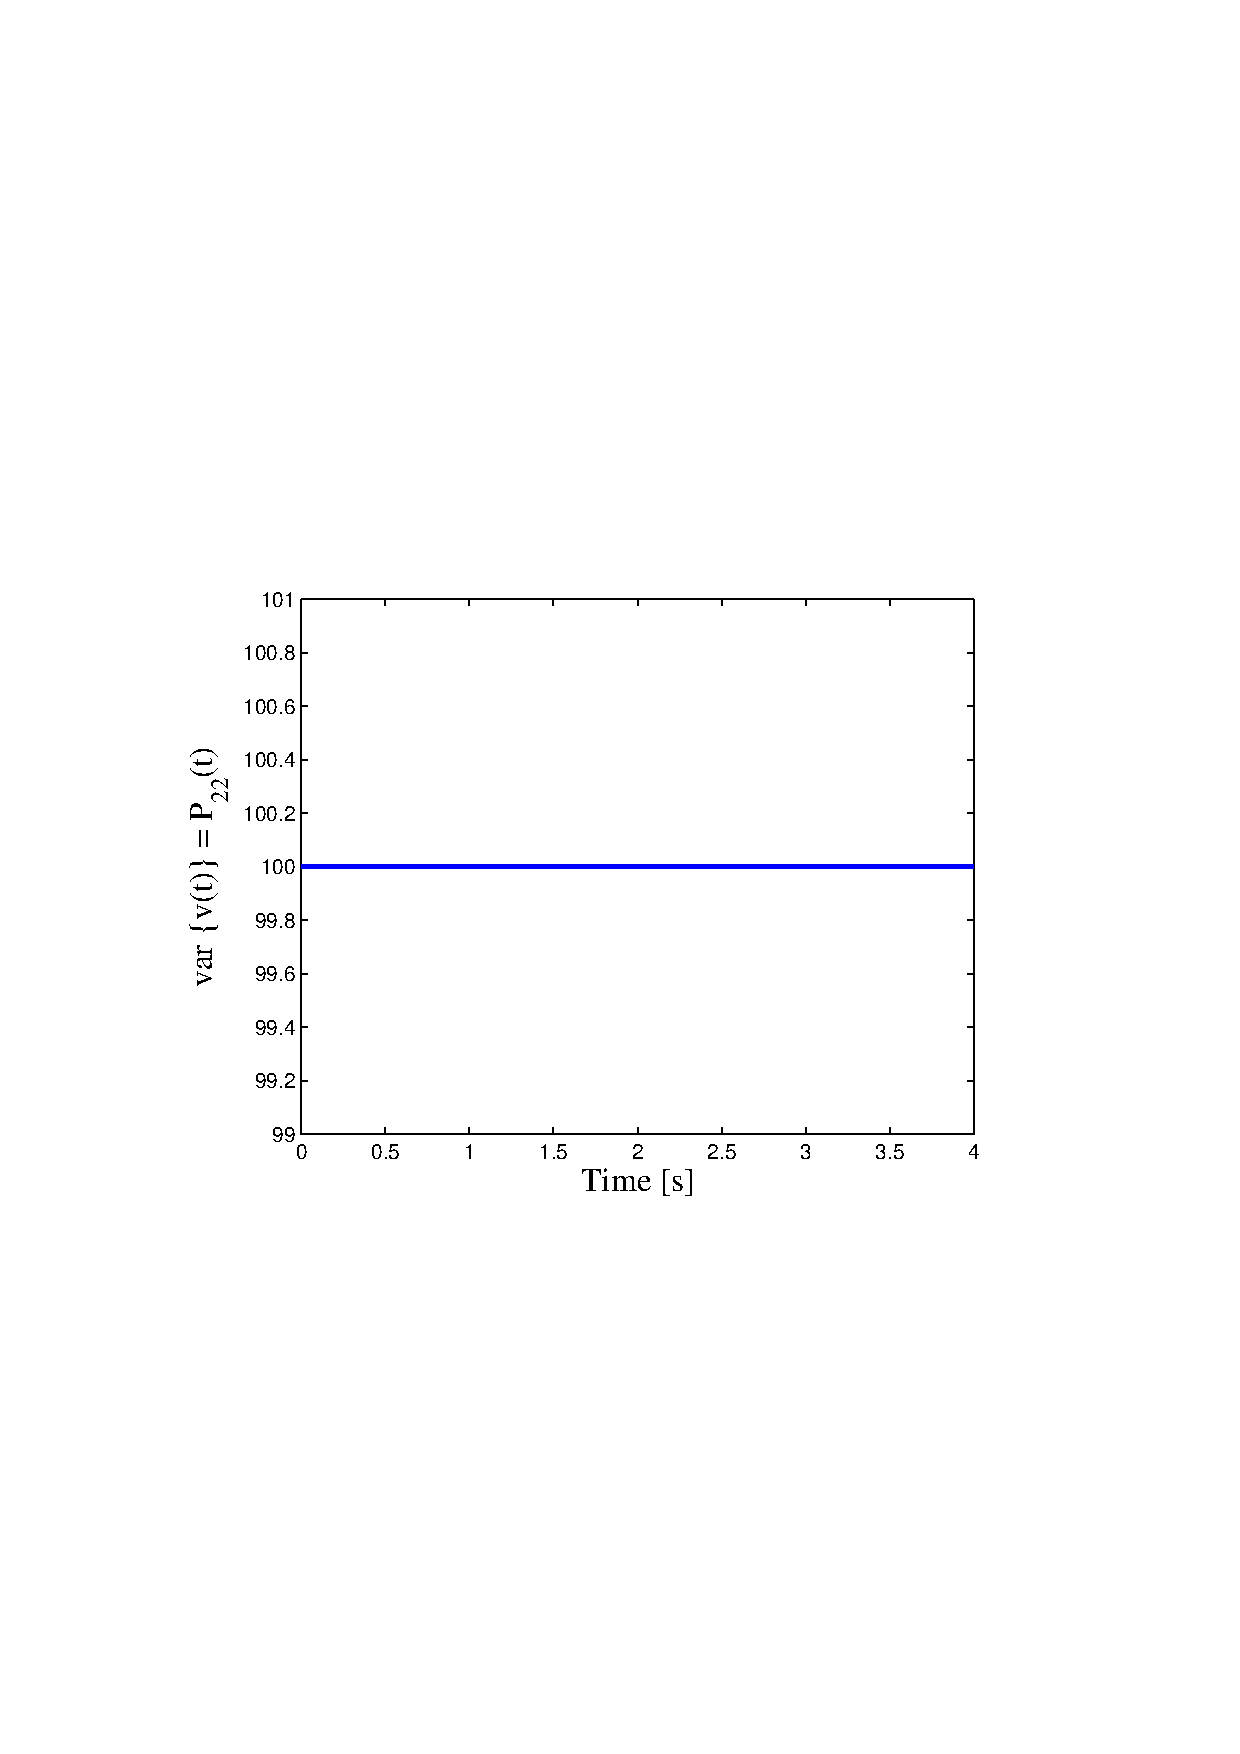
\includegraphics[scale=0.5]{figure/hw4_varv.jpg}
	\caption{The evolution of variance of $ v(t) $}
\end{center}
\end{figure}
\noindent From the sub-equation of equation 18, the differential of the variance of $v(t)$:
\begin{equation}
	\dot P_{22}  =  - 4P_{22}  + 400
\end{equation}
and, at steady state, when $\dot{P_{22}}=0$, I get:
\begin{equation}
	P_{22}  = 100
\end{equation}
Because our initial condition set $P_{22}(0)=P_{22}(infty)$, the value of $P_{22}$ will always be 100 as figure 4.\\

\noindent For the covariance of $s(t)$ and $v(t)$:
\begin{figure}[H]
\begin{center}
	\includegraphics[scale=0.5]{figure/hw4_covsv.jpg}
	\caption{The evolution of covariance of $s(t), v(t)$}
\end{center}
\end{figure}

\noindent From the sub-equation of 18, the differential of the covariance of $s(t)$ and $v(t)$:
\begin{equation}
	\dot P_{12}  =  - 2P_{12}  + P_{22} 
\end{equation}
and, at steady state, when $\dot{P_{12}}=0$, I get:
\begin{equation}
	P_{12}  = \frac{1}{2}P_{22}  = 50
\end{equation}
It shows that, at steady state, the covariance of $s(t)$ and $v(t)$ will converge to 50 as figure 5.

\end{document}
